% version: August 28, 2011

\documentclass{mitpress}
\usepackage{graphicx}


%% Bibliography style %%%%%%%%%%%

%% For Chicago style bibliography style, uncomment:

 \usepackage{natbib}
 \bibliographystyle{chicago}

%% To use APA style bibliography, comment out above
%% and uncomment this:

%% \usepackage[nosectionbib]{apacite}
%% \bibliographystyle{apacite}

%% Index %%%%%%%%%%%%%%%%%%%%%%%%

%% Uncomment to make index:
\usepackage{makeidx}
\makeindex

%%%%%%%%%%%%%%

%%%%%%%%%%%%%%%%%%%%%%%%%%%%%%%%%
%%% Set up Before Text Starts %%%

\title{Perspectives on Free and Open Source Software}
\subtitle{Subtitle Possible}

\bookauthor{Joseph Feller}

\dedication{
Dedication\\
-- initials

(This space may instead be used for an epigraph)
}

%% if appropriate, put Compositor name and address here:
\compositor{}

%% Series Page
\seriespage{
{\bf The MIT Press Free Software Series}

\title{First Book}
\author{author or authors}

\title{Second Book}
\author{author or authors}

}

%% if you want your sections to be numbered, uncomment
%\setcounter{secnumdepth}{3}

%%% End Set Up                %%%
%%%%%%%%%%%%%%%%%%%%%%%%%%%%%%%%%



\begin{document}

%% Title pages and Contents will not print unless this command is used:

\titlepages 


\begin{foreword}
\author{Michael Cusumano}

As with other researchers and authors who study the software business
and software engineering, I have had many opportunities to learn about
free and open source software (FOSS). There is a lot to know, and I am
especially pleased to see this volume of essays from MIT Press because
it provides so much information---both quantitative and qualitative---%
on so many aspects of the open source movement. It will answer many
questions as well as continue to inspire more research for years to
come.

\authoraddress{
Michael Cusumano\\
Groton and Cambridge, Massachusetts\\
February 2005\\
}

(Foreword should be written by someone other than author of book)
\end{foreword}


\begin{seriesforeword}
\author{Author of Series Foreword}

Introduction to this book as part of a series, if appropriate.
\authoraddress{
Author of Series Foreword\\
Address\\
Current Date\\
}
\end{seriesforeword}


\begin{preface}
This is a sample preface. The preface should only
be written by the author of the book.

\authoraddress{
Author of Book\\
Address\\
Current Date\\
}
\end{preface}


\begin{acknowledgment}
We would like to express our sincere thanks to Bob Prior and to the whole
editorial staff at The MIT Press, for their professionalism and support
throughout the process. We would also like to express our appreciation to
the many contributors in this volume. This work would not have been possible
without their passion for scholarship and research.

Most of all, we are grateful to the individuals, communities, and firms
that constitute the free and open source software movements. Their innovations
have challenged our ``common knowledge'' of software engineering,
of organizations and organizing, of the software industry, and of
software as a component of contemporary society.

\authorinitials{JF, BF, SAH, and KRL}

(Acknowledgments can optionally be included in preface, instead of
being in their own section.)
\end{acknowledgment}


\begin{introduction}
\author{Joseph Feller}

\section*{What This Book Is About}
Briefly stated, the terms ``free software'' and ``open source software'' refer
to software products distributed under terms that allow users to:

\begin{itemize}

\item Use the software

\item Modify the software

\item Redistribute the software
\end{itemize}
in any manner they see fit, without requiring that they pay the author(s)
of the software a royalty or fee for engaging in the listed activities. In
general, such terms of distribution also protect what the publishing world
calls the ``moral right'' of the software's author(s) to be identified as such.

Products such as the GNU/Linux operating system, the Apache Web server,
the Mozilla Web browser, the PHP programming language, and the
OpenOffice productivity suite are all well-known examples of this kind of
software.

More detailed, formal definitions for the terms {\it free} and {\it
open source} are
maintained---and vigilantly watch-dogged---by the Free Software Foundation
(FSF)\footnote{http://www.gnu.org/philosophy/free-sw.html.}
 and Open Source Initiative (OSI).\footnote{http://www.opensource.org/docs/definition.php.} However, the definitions are
substantively identical, and the decision to use one of these terms rather
than the other is generally ideological, rather than functional; the FSF
prefers the use of a term that explicitly refers to freedom, while the OSI
believes that the dual meaning of the English word ``free'' 
({\it gratis} or {\it libertas})
is confusing, and instead prefers the emphasis on the availability and
modifiability of source code.\footnote{See Feller and Fitzgerald (2002)
for a fuller discussion of this. Several of the 
chapters in this book also address the issue, directly or indirectly.}

In Europe the French-English construct libre
software has been widely adopted to unambiguously capture the connotation
intended by the FSF.\footnote{You'll find all three terms
(and every possible combination) used by the various authors
whoe wrote the chapters in this book---we let people choose their
own labels, rather than normalizing the book with unintentional
side effects.}

The earliest research and analysis on F/OSS emerged from
within:
\begin{itemize}
\item
The F/OSS community itself (including the writings of Richard M.
Stallman and Eric S. Raymond)

\item
The technology press (for example Wired magazine, O�Reilly and Associates)

\item
 The software engineering research community (for example the ACM and
IEEE)
\end{itemize}
It didn't take long, however, for a substantial and well-rounded literature
to emerge---one addressing F/OSS as not only a software engineering phenomenon,
but as psychological, philosophical, social, cultural, political,
economic, and managerial phenomena as well. The bibliography of this
book\footnote{Most of the publicly available references 
in the bibliography of
this book can be found in multiple citation management formats (EndNote,
Bibtex, and so on) at http://opensource.ucc.ie. Additionally, full-text
versions of many of the papers cited are also available in the research
repository at http://opensource.mit.edu.  We hope that these two resources
will be very valuable to our readers.}
is testament to the variety and richness of this scholarship.

%% Need this command to make endnotes appear. Should be at end
%% of every chapter or introduction where \footnote{} is used.

\endnotes

\end{introduction}




\part{Motivation in Free/Open Source Software Development}

%% version of title in square brackets goes to table of contents

\chapter[Why Hackers Do What They Do:
Understanding Motivation and Effort in Free/Open Source Software
Projects]
{Why Hackers Do What They Do:\\ Understanding
Motivation and Effort in Free/Open Source Software
Projects}


``What drives Free/Open Source software (F/OSS) developers to contribute
their time and effort to the creation of free software products?'' 
is a question
often posed by software industry executives, managers, and academics
when they are trying to understand the relative success of the F/OSS movement.
Many are puzzled by what appears to be irrational and altruistic
behavior by movement participants: giving code away, revealing proprietary
information, and helping strangers solve their technical problems.

\section{Enjoyment-based Intrinsic Motivation} 
Having fun or enjoying oneself
when taking part in an activity is at the core of the idea of intrinsic
motivation (Deci and Ryan 1985). 

Csikszentmihalyi (1975) was one of the first
psychologists to study the enjoyment dimension. He emphasized that
some activities were pursued for the sake of the enjoyment derived from
doing them. He proposed a state of ``flow,'' in which enjoyment is maximized,
characterized by intense and focused concentration; a merging of
action and awareness; confidence in one's ability; and the enjoyment of
the activity itself regardless of the outcome (Nakamura and Csikszentmihalyi
2003). 

\subsection{Community Identification}
In F/OSS projects, we see a strong sense of community identification and
adherence to norms of behavior. Participants in the F/OSS movement
exhibit strong collective identities. 

\subsubsection{The New Hacker's Dictionary}
Canonical texts like The New Hacker's
Dictionary (Raymond 1996), The Cathedral and the Bazaar (Raymond 2001),
and the GNU General Public License (GPL) (Stallman 1999a) have created
shared meaning about the individual and collective identities of the
hacker2 culture and the responsibilities of membership within it. Indeed,
the term hacker is a badge of honor within the F/OSS community, as
opposed to its pejorative use in popular media. The hacker identity
includes solving programming problems, having fun, and sharing code at
the same time. Private gain-seeking within the community is minimized
by adherence to software licenses like the GPL and its derivatives, which
allow for user rights to source code and subsequent modification.


\begin{enumerate} 
\item In the sealed-bid auction, everyone submits a
sealed envelope containing their bid. The auctioneer opens them and
awards the contract to the highest bidder.

\item In the English auction, the
auctioneer starts out the bidding at somereserve price, and keeps on
raising it until one bidder remains, who is thewinner. The effect of
this is that the bidder who places the highest valuation on the
contract wins, but at the valuation of the next-highest bidder(plus
the bid increment).

\item
The all-pay auction is similar to the English
auction, except that at eachround all the bidders have to pay the
current price. Eventually, there isonly one bidder left, who gets the
contract' but the losers don't get a refund. (This scheme models
what happens in litigation, or in a symmetric war of attrition.)
\end{enumerate}

%% \callout{} shows where this figure should appear. 
%% (Figures and Tables must be sent to end of chapter)

\callout{Figure 1.1}

It is remarkable that large numbers of people manage to work
together successfully to create high-quality, widely used products. Our first
set of questions (Q1 to Q4) is aimed at understanding basic parameters of
the process by which Apache and Mozilla came to exist.

\begin{description}
\item[Q1:]What were the processes used to develop Apache and Mozilla?
In answer to this question, we construct brief qualitative descriptions of
the Apache and Mozilla development processes.

\item[Q2:]How many people wrote code for new functionality? How many people
reported problems? How many people repaired defects?
We want to see how large the development communities were, and
identify how many people actually occupied each of these traditional
development and support roles.

\item[Q3:]Were these functions carried out by distinct groups of people? That
is, did people primarily assume a single role? Did large numbers of people
participate somewhat equally in these activities, or did a small number of
people do most of the work?

\end{description}
Within each development community, what division of labor resulted
from the OSS ``people choose the work they do'' policy? We want to construct
a profile of participation in the ongoing work.

%% \callout{} shows where this table should appear. 
%% (Figures and Tables must be sent to end of chapter)

\callout{Table 1.1}

In particular, the probability $E$ of a security
failure at time $t$, at which time $n$ bugs have been
removed, is
\begin{equation}
E=\sum^{\infty}_{i=n+1} d^{-E_jt}\sim K/t
\end{equation}
over a wide range of values of $t$.

%% Instead of endnotes, use \note for short comment

\note
I got useful comments from Rob Brady, Hal Varian,
Jacques Cr\'emer, Peter Bishop, Richard Clayton, Paul
Leach, and many others.

%% For single endnote use \note and \endnote{<num>}{<text>}
\note
\endnote{1}{See the COTS-Based Systems (CBS) Iniative Web site
at http://www.sei.cmu.eud/cbs.}

\newpage
%% name your figure files with figure_(chapter)_(figure number)

\begin{figure}
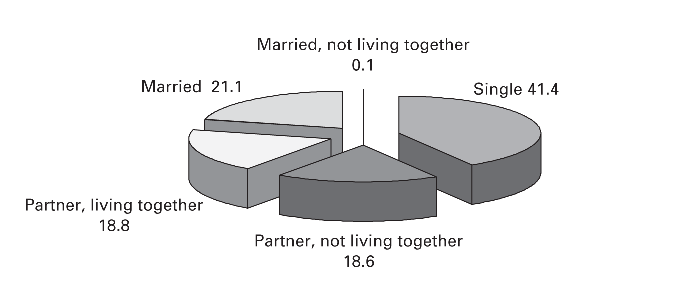
\includegraphics[width=.7\textwidth]{figure_01_01}
\caption{Civil status of developers.
In the absence of clear monetary transactions, the interplay of contribution
and return can be described in the form of `balanced value flow'
where one assumes rational self-interest but allows that self-interest can
include a range of different types of reward, not just monetary
compensation.}  
\end{figure}

\begin{table}
\caption{General characteristics of survey respondents}
\centerline{
\begin{tabular}{@{}p{2in}crccc@{}}
\hline
Variable &Obs& Mean& Std. Dev.& Min\ \ \ & Max\\
\hline
Age& 677.00& 29.80& 7.95& \llap{1}4.00& 56.00\\
Years programming &673.00& 11.86 &7.04& 1.00& 44.00\\
Current F/OSS projects& 678.00& 2.63& 2.14& 0.00& 20.00\\
All F/OSS projects &652.00 &4.95 &4.04& 1.00& 20.00\\
Years since first contribution
to F/OSS community
& 683.00& 5.31& 4.34& 0.00& 21.00\\
\hline
\end{tabular}
}
\end{table}


\chapter{Epigrams and Quotations}


%% \epigram{<text>}{<author>}
\epigram{There is a tremendous sense of satisfaction to the 
``see bug, fix bug, see
bug fix get incorporated so that the fix helps others'' cycle.}
{FreeBSD developer}

\section{Example of Short Quotation}
As Tim O'Reilly wrote in his essay 
{\it Hardware, Software and Infoware} (O'Reilly
1997, 192--193):

%%\begin{quote}...\end{quote} for short quote, one paragraph:

\begin{quote} If you look at a large web site like Yahoo!, you'll see that
behind the scenes, an army of administrators and programmers are continually
rebuilding the product. Dynamic content isn't just automatically
generated, it is also often hand-tailored, typically using an array of quick
and dirty scripting tools.  
\end{quote}

``We don't create content at Yahoo! We
aggregate it,'' says Jeffrey Friedl, author of the book {\it
Mastering Regular
Expressions} and a full-time Perl programmer at Yahoo.  

\section{Example of Long Quotation}

This can be exemplified by the rhetoric of different movement
intellectuals, as with the polemic between Eric Raymond and Richard Stallman,
founder and leader of the free software movement from which open
source grew.

Stallman, a hacker formerly at MIT, has positioned himself as one of the
most prominent activist within the programming community, with large
contributions to free software, his GNU/Linux project, for example, and
as the founder of the Free Software Foundation (FSF). Stallman always
adopted a more ideological line in his work with free software, promoting
the freedom of hacking and information, than that found in the open
source movement. Taking a look at his personal website, his political interest
in different ``freedom of speech'' ---and in the civil rights movements---are 
evident. However, Raymond has a more pragmatic outlook, which
maybe is best explained via a well-known dispute between Raymond and
Stallman, initiated by a posting from Stallman to an Internet bulletin
board:

%%\begin{quotation}...\end{quotation} for long quote, more than one paragraph

\begin{quotation}
People have been speaking of me in the context of the Open Source movement.
That's misleading, because I am not a member of it. I belong to the Free
Software movement. 

In this movement we talk about freedom, about principle, about the rights
that computer users are entitled to. The Open Source movement avoids talking
about those issues, and that is why I am not joining it. The two movements
can work together on software\ldots But we disagree on the basic issues. 

\noindent
(Stallman 1999b)
\end{quotation}

Raymond responded with an essay where he stated that he could agree
on Stallman's ideas about freedom and rights, but that it was ineffective
and bad tactics for the free software community to engage in those issues:

\begin{quotation}
OSI's tactics work [. . .] FSM's tactics don't work, and never did. [sic!]
RMS's [Richard
Matthew Stallman] best propaganda has always been his hacking. 

So it is for all of us; to the rest of the world outside our little tribe,
the excellence of our software is a far more persuasive argument for openness
and freedom than any amount of highfalutin appeal to abstract principles. So
the next time RMS, or anybody else, urges you to ``talk about freedom,''
I urge you to reply ``Shut up and show them the code.''

\noindent
(Raymond 1999b)
\end{quotation}

Though the open source and free software movements share an ambition
to create free software of high quality, and share mutual cultural
expressions through the hacker community, this is an example of a power
struggle where the leaders take different roles as symbolic organizers. It is
a battle that originates from different perspectives on how work should be
done and what the strategies are to be. Most importantly, this inspires
members to act on different forces and purposes when contributing to the
movement.






\chapter{Sample Citations}

(From the MIT Press website):\\
If you use the author-date citation system, include the citation within the text, and make sure the source appears in the reference list. For example:

\begin{quote}
Rowe claims that ``the role of the designer . . . in such a complex system is one of describing modes of interaction and degrees of freedom within and between multiple agents'' (Rowe 2001, 373).

\noindent
or

Rowe (2001, 273) claims that ``the role of the designer . . . in such a complex system is one of describing modes of interaction and degrees of freedom within and between multiple agents.''
\end{quote}

\begin{description}
\item[Natbib]
If you are using natbib with the chicago bibliography style, 
you would get these results by typing\\
\verb+\citep{knuth79}+ to produce (Knuth, 1979), and
\verb+\cite{knuth79}+ to produce Knuth (1979).

If you want to refer to the page number,\\ 
\verb+\citep[79]{knuth79}+ will produce (Knuth 1979, 79)\\
or to put the parens around only the year
and pagenumber, \verb+\citet[79]{knuth79}+, will produce Knuth (1979, 79).

\item[Apacite]
If you are using apacite, you would get these results by typing
\verb+\cite{knuth79}+ will produce (Knuth, 1979), and\\
\verb+\citeA{knuth79}+ will produce Knuth (1979).

If you want to refer to the page number,\\
\verb+\cite[79]{knuth79}+ (Knuth, 1979, 79).\\
or to put the parens around only the year
and pagenumber,\\ 
\verb+\citeA[79]{knuth79}+, Knuth (1979, 79).

\end{description}

Of course you will want to adopt a consistent citation form.

\section{Useful \LaTeX\ References}
Of course, the beloved hero of all \LaTeX\ users is Donald Knuth,
the author of \TeX\ which underlies all the code of our
typesetting system. \cite{knuth79} is his seminal
book on the topic. 

For a concise list of \LaTeX\ commands, the book by its
original author, Leslie Lamport, \cite{lamport94}
will be most helpful.
A more compreshensive book for beginning \LaTeX\ users is by
Goossens, Mittlebach, and Samarin, \cite{goossens93}.
For information about \LaTeX\ and graphics, 
\cite[255]{rahtz89}, provides an important source.

If you are looking for information on Bib\TeX, you'll
find \cite{patashnik88} a good source, included in
the \TeX\ distribution.

Finally, George D. Greenwade has written a description of
CTAN, the Comprehensive TeX Archive Network, \cite{greenwade93}.

\chapter{Index Steps}
\begin{enumerate}
\item
 Uncomment before \verb+\begin{document}+\\
\verb+   \usepackage{makeidx}+\\
\verb+   \makeindex+


\item
Enter \verb+\index{term}+ or \verb+\index{term!subterm}+ 
or \verb+\index{term!subterm!subterm}+

Be Careful!  no spaces before or after the !, or your sub terms will
not alphabetize correctly.

\item
 Run LaTeX, producing filename .idx

\item
Then, on the command line, type `makeindx filename' which will
     produce filename.ind. You can edit this file if you want to change
     anything in it.

\item Now, index will appear where you type this command:\\
\verb+\printindex+
\end{enumerate}

You will find more information in our documentation,\\
MITPressLaTeXManuscript.pdf.


%%% End Matter %%%%



\begin{epilogue}
\title{Epilogue: Open Source outside the Domain of Software}
\author{Clay Shirky}

The unenviable burden of providing an epilogue to Perspectives on Free and
Open Source Software is made a bit lighter by the obvious impossibility of
easy summation. The breadth and excellence of the work contained here
makes the most important point: the patterns implicit in the production
of Open Source software are more broadly applicable than many of us
believed even five years ago. Even Robert Glass, the most determined Open
Source naysayer represented here, reluctantly concludes that ``[T]here is no
sign of the movement's collapse because it is impractical.''

So the publication of this book is a marker---we have gotten to a
point where we can now take at least the basic success of the Open
Source method for granted. This is in itself a big step, since much of the
early literature concerned whether it could work at all. Since even many
of its critics now admit its practicality, one obvious set of questions is how
to make it work better, so that code produced in this way is more useful,
more easily integrated into existing systems, more user-friendly, more
secure.

\end{epilogue}

\appendix
\chapter{Here is an Appendix}
\author{Appendix Author}
Appendix text here.

%%%%%%%%%%%%%%%%%%%%%%%%%%%%%%%%%%%%%%%%%%%%%%%%%%%%%%%%%%%%%
%%% References

%%% If, instead of using BibTeX, you want to enter your own bib entries, 
%%% follow this form, giving the author-year in the optional square
%%% bracket after \bibitem. This will make the cite produce the
%%% correct author date form: \cite{rowe} will produce (Rowe, 2011).
%%% Please use italics for book titles.

%%
% \begin{thebibliography}{Nahas, 1999} %% put widest term here to determine
                                       %% width of bibliography margin.
%bookcd
% \bibitem[Rowe, 2011]{rowe}
% Rowe, Robert. 2001. Machine Musicianship. Cambridge, Mass.: MIT Press.

%Chapter in a Book
% \bibitem[Marx, 1988]{marx}
% Marx, Leo. 1988. ``The railroad-in-the landscape: An iconological reading 
% of a
% theme in American art.'' In {\it The railroad in American art: Representations of
% technological change}, ed. Susan Danly and Leo Marx, 170--196. Cambridge,
% Mass.: MIT Press.

%Article in a Journal
% \bibitem[Nahas, 1999]{nahas}
% Nahas, Ronald C. 1999. ``Beirut rising.'' Urban Land 58 (10) (October):
% 40--46. 
% \end{thebibliography}
%%%%%%%%%%%%%%%%%%%%%%%%%%%%%%%%%%


%%%%% Bibliography using bibtex. 

% \bibliography{<filename.bib>} will
% access filename.bib for bibliography database. After you run LaTeX
% on your filename.tex file once, you can run bibtex on filename,
% then run LaTeX on filename twice to make the bibliography, and to
% update the citations.

\bibliography{sample}

%%%%% List of Contributors
\listofcontributors

\section*{About the Editors}


\name{Joseph Feller PhD} is a Senior Lecturer in Business Information Systems
at University College Cork, Ireland. He has chaired the annual international
Open Source Software Engineering workshop series since it was established at
ICSE in 2001. He is the coauthor, with Brain Fitzgerald, of Understanding
Open Source Software Development (Addison-Wesley, 2002). His research on
free/open source software has been presented in international journals and
conference proceedings, and he has served as guest editor (again with
Fitzgerald) for F/OSS special issues of Information Systems Journal, IEE
Proceedings: Software (with Andre van der Hoek), and Syst\`emes
d'Information et Management (with Frederic Adam). Joseph received his PhD
from UCC, and a BA from American University.

\name{
Brian Fitzgerald} holds the endowed Frederick A. Krehbiel II Chair in
Innovation in Global Business and Technology, at the University of
Limerick, Ireland, where he is also a research fellow and a Science Foundation
Ireland investigator. He has a PhD from the University of London and
has held positions at University College Cork, Ireland, Northern Illinois
University, U.S., the University of Gothenburg, Sweden, and Northumbria
University, UK. His publications include seven books and more than 60
papers published in leading international conferences and journals. Having
worked in the industry prior to taking up an academic position, he has
more than 20 years experience in the IS field.


\section*{About the Contributors}

\name{
Philippe Aigrain} is the founder and CEO of the Society for Public Information
Spaces (www.sopinspace.com), a venture specializing in free software
tools and services for Internet-based public debate on policy issues.
Prior to that, he worked for the Information Society DG of the European
Commission where he coordinated actions related to F/OSS until April
2003. He was trained as a mathematician and computer scientist, and has
researched subjects such as compilers, interaction with audiovisual media,
and the sociology of information exchanges.

\name{
Ross Anderson} was one of the founders of the study of information security
economics and chairs the Foundation for Information Policy Research.
A fellow of the IEE, he was also one of the pioneers of peer-to-peer systems,
of API attacks on cryptographic processors, and of the study of hardware
tamper-resistance. He was one of the inventors of Serpent, a finalist in the
competition to find an advanced encryption standard. 


%%%%%%%%%%%%%%%%%%%%%%%%%%
%%% Index will appear here 

%% Index steps: 
%% 1. Uncomment before \begin{document}
%%    \usepackage{makeidx}
%%    \makeindex

%% 2. Enter \index{term} or \index{term!subterm} \index{term!subterm!subterm}
%%    (no spaces before or after the !)

%% 3. Run LaTeX, producing filename .idx

%% 4. Then on command line type `makeindx filename' which will
%%     produce filename.ind. You can edit this file if you want to change
%%     anything in it.

%% 5. Now, index will appear where you type this command:

\printindex

\end{document}
